\chapter{Architecture} \label{cap:architecture}

Kloud Motors follows a microservices architecture implemented in Go. The public surface of the application is a REST and WebSocket gateway, while the internal services communicate through gRPC. The same service decomposition is used for local execution with Docker Compose and for cloud execution on Kubernetes.

\section{Application Architecture}

At application level, the platform is organised around a single gateway and a set of domain services. Clients do not call the internal services directly. Instead, all HTTP routes under \texttt{/api} and all public WebSocket routes are received by the gateway. The gateway validates requests, verifies Firebase ID tokens for protected operations, maps HTTP requests into gRPC calls, and proxies WebSocket connections for chat and auctions.

The main application services are:

\begin{itemize}
    \item \textbf{Gateway service}: exposes the REST API, WebSocket entry points, health endpoint, metrics endpoint, Firebase token validation, and gRPC clients for downstream services.
    \item \textbf{Listing service}: owns listing details, listing summaries, comparison, listing creation, update, deletion, ownership checks, and sold state checks.
    \item \textbf{Search service}: provides paginated listing search over the listing database and caches repeated search results in Redis.
    \item \textbf{Market price service}: computes average, minimum, and maximum market prices for a selected brand and model.
    \item \textbf{Geographical market insights service}: provides aggregate, price-comparison, and by-location statistics grouped by district, city, or country.
    \item \textbf{User service}: handles Firebase-backed registration, login, token refresh, internal user resolution, user previews, and favourite listings.
    \item \textbf{Seller service}: provides seller profiles and seller previews.
    \item \textbf{Chat service}: manages chat creation, chat listing, chat history, and live buyer-seller messaging.
    \item \textbf{Auction service}: manages auction listing, creation, detail retrieval, deletion, bidding, bid retrieval, and live auction updates.
\end{itemize}

The application data is separated by concern. The listing database is shared by read heavy marketplace services because listing, search, market price, and geographical insights all operate over the same vehicle data. User, seller, chat, and auction state are stored in separate PostgreSQL databases. Chat also uses Firestore for message persistence when configured. Redis is used as a cache aside layer for listing detail, listing summary, and search query results. Google Pub/Sub is used by chat and auction services to distribute real-time WebSocket events across replicas.

\section{Technical Architecture}

The services are containerised and deployed to Kubernetes under the \texttt{vehicles-prod} namespace. The top-level Kustomize configuration includes the namespace, shared service account, Cloud SQL configuration, gateway, all domain services, Redis, backup resources, and ingress. The ingress accepts traffic for \texttt{kloud-motors.com} and routes \texttt{/api/}, \texttt{/api/chat/ws/}, and \texttt{/api
/auctions/ws/} to the gateway service.

Inside Kubernetes, service discovery is performed through Kubernetes service names. The gateway receives downstream addresses from its ConfigMap, including \texttt{listing-service:50054}, \texttt{search-service:50056}, \texttt{user-service:50058}, \texttt{seller-service:50057}, \texttt{chat-service:50052}, \texttt{marketprice-service:50055}, \texttt{geographic-market-insights-service:50053}, and \texttt{auction-
service:50051}. WebSocket upstreams are configured separately as \texttt{ws://chat-service:8080} and \texttt{ws://auction-service:8081}. Several cross-cutting technical mechanisms are implemented in the codebase:

\begin{itemize}
    \item \textbf{Authentication}: the user service calls Firebase Identity Toolkit and Secure Token APIs for registration, login, and refresh. The gateway verifies Firebase ID tokens and resolves them to internal user IDs.
    \item \textbf{Resilience}: the gateway wraps downstream gRPC clients with circuit breakers. Chat and auction also wrap selected listing and seller service calls with circuit breakers.
    \item \textbf{Observability}: the gateway exposes \texttt{/metrics} for Prometheus and \texttt{/api/health} for health checks. HTTP and gRPC boundaries are instrumented with OpenTelemetry in the gateway and main services.
    \item \textbf{Scalability}: services have Kubernetes deployment and service manifests, and scalable services define HorizontalPodAutoscaler resources. Redis reduces database load for repeated read paths, while Pub/Sub enables horizontally scaled WebSocket delivery.
    \item \textbf{Backup}: a Kubernetes CronJob exports configured Cloud SQL databases to Google Cloud Storage.
    \item \textbf{Infrastructure as code}: Terraform defines core GCP resources, including Cloud SQL, a backup bucket, Artifact Registry, Pub/Sub topics, service accounts, VPC networking, and GKE resources.
    \item \textbf{Automation}: GitHub Actions runs Go unit tests, Docker Compose based integration tests, and Terraform validation/deployment workflows.
\end{itemize}

\section{Architecture Diagram}

Figure~\ref{fig:architecture} summarises the connection between the client, gateway, services, data stores, messaging infrastructure, observability stack, deployment automation, and cloud infrastructure.

\begin{figure}[p]
    \centering
    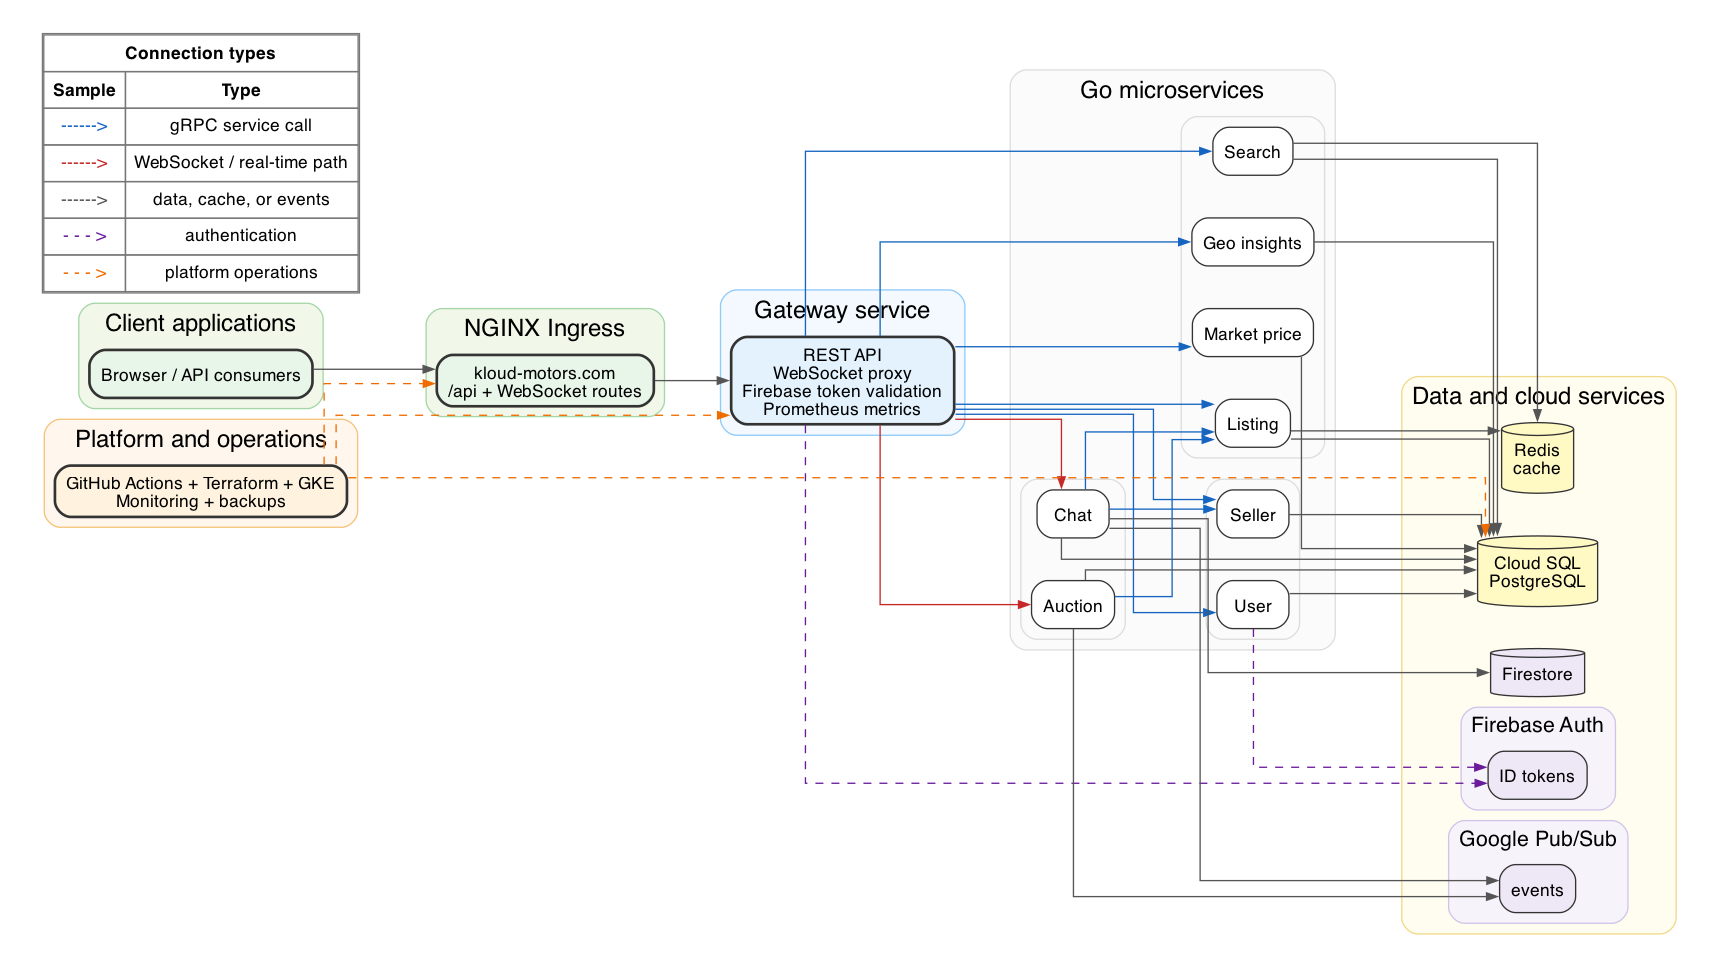
\includegraphics[angle=90,width=\textwidth,height=0.78\textheight,keepaspectratio]{architecture/images/architecture.png}
    \caption{Kloud Motors application and technical architecture}
    \label{fig:architecture}
\end{figure}
